\definecolor{opdrachtkleur}{RGB}{204,0,0} %Initialiseer op RUG-rood
\definecolor{J1H2}{RGB}{204,102,0}
\definecolor{J2H6}{RGB}{132,133,255}
\definecolor{J3H5}{RGB}{175,0,175}

\lstset{
	keepspaces=true,
	frame=tBlR,
	rulesepcolor=\color{opdrachtkleur},
	numbers=left,
	tabsize=2,
	breaklines=true,
	breakatwhitespace=true,
	captionpos=b,
	postbreak={\mbox{$\cdots$}},
	prebreak={\mbox{$\cdots$}},
	mathescape=true,%
	}
	
\def\pijl{
	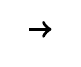
\begin{tikzpicture}[very thick,x=1em,y=1em,baseline={(0,-0.35em)}]
		\draw [->](-0.4,0) -- (0.4,0);
	\end{tikzpicture}
	}
\def\eindpijl{
	
\begin{tikzpicture}[very thick,x=1em,y=1em,baseline={(0,-0.3em)}]
		\draw[<-] (-0.25,0) -- (0.25,0) -- (0.25,0.3); 
	\end{tikzpicture}
	}
\def\vervolg{
	
\begin{tikzpicture}[very thick,x=1em,y=1em,baseline={(0,-0.3em)}]
		\draw[<-] (0.25,0) -- (-0.25,0) -- (-0.25,0.3); 
	\end{tikzpicture}%
	}
\def\dakje{
	
\begin{tikzpicture}[very thick,x=1em,y=1em,baseline={(0,0)}]
		\draw (-0.3,0.3) -- (0,0.7) -- (0.3,0.3);
	\end{tikzpicture}
	}
\def\dh{
	
\begin{tikzpicture}[very thick,x=1em,y=1em,baseline={(0,0)}]
		\filldraw (0,0) -- (0.3,0) -- (0.3,0.3) -- cycle;
	\end{tikzpicture}
	}
\def\sp{\bfseries\textvisiblespace}
\lstdefinestyle{basic}{%
	language=[Visual]Basic,%
	keywordstyle=\bfseries\underbar,%
	commentstyle=\itshape\small,%
	mathescape=true,%
	morekeywords={To,LpWhile,IfEnd,Step,Lbl,Locate,ClrText},%
	literate={->}{\pijl}1 {;}{\eindpijl}1{^}{\dakje}1{;;}{\dh}1%
	}
	
\lstdefinestyle{pascal}{%
	language=Pascal,
	keywordstyle=\bfseries\underbar,%
	commentstyle=\itshape\small,%
	mathescape=true,%
	deletekeywords=[1]{mod,false},%
	morekeywords={RETURN,EXPORT,LOCAL,FROM},
	morecomment=[l]{//},
}

\lstdefinelanguage{pseudo}
{
  % list of keywords
  morekeywords={invoer,uitvoer,voor,als,dan,anders,geef,print,zolang,zeg},
  sensitive=false, % keywords are not case-sensitive
  morecomment=[l]{//}, % l is for line comment
  morecomment=[s]{/*}{*/}, % s is for start and end delimiter
  morestring=[b]" % defines that strings are enclosed in double quotes
}

\def\lstsqrt#1{\raisebox{3pt}[\totalheight][0pt]{$\smash{\sqrt{#1}}$}}
